% Options for packages loaded elsewhere
\PassOptionsToPackage{unicode}{hyperref}
\PassOptionsToPackage{hyphens}{url}
\PassOptionsToPackage{dvipsnames,svgnames,x11names}{xcolor}
%
\documentclass[
  letterpaper,
  DIV=11,
  numbers=noendperiod]{scrreprt}

\usepackage{amsmath,amssymb}
\usepackage{lmodern}
\usepackage{iftex}
\ifPDFTeX
  \usepackage[T1]{fontenc}
  \usepackage[utf8]{inputenc}
  \usepackage{textcomp} % provide euro and other symbols
\else % if luatex or xetex
  \usepackage{unicode-math}
  \defaultfontfeatures{Scale=MatchLowercase}
  \defaultfontfeatures[\rmfamily]{Ligatures=TeX,Scale=1}
\fi
% Use upquote if available, for straight quotes in verbatim environments
\IfFileExists{upquote.sty}{\usepackage{upquote}}{}
\IfFileExists{microtype.sty}{% use microtype if available
  \usepackage[]{microtype}
  \UseMicrotypeSet[protrusion]{basicmath} % disable protrusion for tt fonts
}{}
\makeatletter
\@ifundefined{KOMAClassName}{% if non-KOMA class
  \IfFileExists{parskip.sty}{%
    \usepackage{parskip}
  }{% else
    \setlength{\parindent}{0pt}
    \setlength{\parskip}{6pt plus 2pt minus 1pt}}
}{% if KOMA class
  \KOMAoptions{parskip=half}}
\makeatother
\usepackage{xcolor}
\setlength{\emergencystretch}{3em} % prevent overfull lines
\setcounter{secnumdepth}{5}
% Make \paragraph and \subparagraph free-standing
\ifx\paragraph\undefined\else
  \let\oldparagraph\paragraph
  \renewcommand{\paragraph}[1]{\oldparagraph{#1}\mbox{}}
\fi
\ifx\subparagraph\undefined\else
  \let\oldsubparagraph\subparagraph
  \renewcommand{\subparagraph}[1]{\oldsubparagraph{#1}\mbox{}}
\fi


\providecommand{\tightlist}{%
  \setlength{\itemsep}{0pt}\setlength{\parskip}{0pt}}\usepackage{longtable,booktabs,array}
\usepackage{calc} % for calculating minipage widths
% Correct order of tables after \paragraph or \subparagraph
\usepackage{etoolbox}
\makeatletter
\patchcmd\longtable{\par}{\if@noskipsec\mbox{}\fi\par}{}{}
\makeatother
% Allow footnotes in longtable head/foot
\IfFileExists{footnotehyper.sty}{\usepackage{footnotehyper}}{\usepackage{footnote}}
\makesavenoteenv{longtable}
\usepackage{graphicx}
\makeatletter
\def\maxwidth{\ifdim\Gin@nat@width>\linewidth\linewidth\else\Gin@nat@width\fi}
\def\maxheight{\ifdim\Gin@nat@height>\textheight\textheight\else\Gin@nat@height\fi}
\makeatother
% Scale images if necessary, so that they will not overflow the page
% margins by default, and it is still possible to overwrite the defaults
% using explicit options in \includegraphics[width, height, ...]{}
\setkeys{Gin}{width=\maxwidth,height=\maxheight,keepaspectratio}
% Set default figure placement to htbp
\makeatletter
\def\fps@figure{htbp}
\makeatother

\KOMAoption{captions}{tableheading}
\makeatletter
\makeatother
\makeatletter
\@ifpackageloaded{bookmark}{}{\usepackage{bookmark}}
\makeatother
\makeatletter
\@ifpackageloaded{caption}{}{\usepackage{caption}}
\AtBeginDocument{%
\ifdefined\contentsname
  \renewcommand*\contentsname{Table of contents}
\else
  \newcommand\contentsname{Table of contents}
\fi
\ifdefined\listfigurename
  \renewcommand*\listfigurename{List of Figures}
\else
  \newcommand\listfigurename{List of Figures}
\fi
\ifdefined\listtablename
  \renewcommand*\listtablename{List of Tables}
\else
  \newcommand\listtablename{List of Tables}
\fi
\ifdefined\figurename
  \renewcommand*\figurename{Figure}
\else
  \newcommand\figurename{Figure}
\fi
\ifdefined\tablename
  \renewcommand*\tablename{Table}
\else
  \newcommand\tablename{Table}
\fi
}
\@ifpackageloaded{float}{}{\usepackage{float}}
\floatstyle{ruled}
\@ifundefined{c@chapter}{\newfloat{codelisting}{h}{lop}}{\newfloat{codelisting}{h}{lop}[chapter]}
\floatname{codelisting}{Listing}
\newcommand*\listoflistings{\listof{codelisting}{List of Listings}}
\makeatother
\makeatletter
\@ifpackageloaded{caption}{}{\usepackage{caption}}
\@ifpackageloaded{subcaption}{}{\usepackage{subcaption}}
\makeatother
\makeatletter
\@ifpackageloaded{tcolorbox}{}{\usepackage[many]{tcolorbox}}
\makeatother
\makeatletter
\@ifundefined{shadecolor}{\definecolor{shadecolor}{rgb}{.97, .97, .97}}
\makeatother
\makeatletter
\makeatother
\ifLuaTeX
  \usepackage{selnolig}  % disable illegal ligatures
\fi
\IfFileExists{bookmark.sty}{\usepackage{bookmark}}{\usepackage{hyperref}}
\IfFileExists{xurl.sty}{\usepackage{xurl}}{} % add URL line breaks if available
\urlstyle{same} % disable monospaced font for URLs
\hypersetup{
  pdftitle={Recipes from our catalogue},
  pdfauthor={Grants},
  colorlinks=true,
  linkcolor={blue},
  filecolor={Maroon},
  citecolor={Blue},
  urlcolor={Blue},
  pdfcreator={LaTeX via pandoc}}

\title{Recipes from our catalogue}
\author{Grants}
\date{12/17/22}

\begin{document}
\maketitle
\ifdefined\Shaded\renewenvironment{Shaded}{\begin{tcolorbox}[breakable, sharp corners, borderline west={3pt}{0pt}{shadecolor}, enhanced, interior hidden, boxrule=0pt, frame hidden]}{\end{tcolorbox}}\fi

\renewcommand*\contentsname{Table of contents}
{
\hypersetup{linkcolor=}
\setcounter{tocdepth}{2}
\tableofcontents
}
\bookmarksetup{startatroot}

\hypertarget{family-recipes}{%
\chapter*{Family Recipes}\label{family-recipes}}
\addcontentsline{toc}{chapter}{Family Recipes}

\markboth{Family Recipes}{Family Recipes}

Recipes from our catalogue

\bookmarksetup{startatroot}

\hypertarget{appetizers}{%
\chapter*{Appetizers}\label{appetizers}}
\addcontentsline{toc}{chapter}{Appetizers}

\markboth{Appetizers}{Appetizers}

\hypertarget{recipe}{%
\section*{Recipe}\label{recipe}}
\addcontentsline{toc}{section}{Recipe}

\markright{Recipe}

\bookmarksetup{startatroot}

\hypertarget{breakfast}{%
\chapter*{Breakfast}\label{breakfast}}
\addcontentsline{toc}{chapter}{Breakfast}

\markboth{Breakfast}{Breakfast}

\hypertarget{daddy-bear-oatmeal}{%
\section*{Daddy Bear Oatmeal}\label{daddy-bear-oatmeal}}
\addcontentsline{toc}{section}{Daddy Bear Oatmeal}

\markright{Daddy Bear Oatmeal}

\begin{itemize}
\tightlist
\item
  1/3 cup old fashion oats (Quaker)
\item
  1/3 cup Bob's thick oats
\item
  1 tablespoon steel cut oats
\item
  1 tablespoon oat groats (optional)
\item
  1 tablespoon millet seed (optional)
\item
  1 teaspoon flax seed (optional)
\end{itemize}

Mix with 1 cup milk (more generous if optional ingredients) in a deep
microwavable bowl (so it won't boil over). Microwave on high for 3 to 3
1/2 minutes, or until reaching a boil. (Stove top cooking is not
recommended.) Cover with a plate and let stand for 30 minutes. Can put
in refrigerator and warm up the next day.

\includegraphics{./assets/oatmealBowl.png}

\hypertarget{scones}{%
\section*{Scones}\label{scones}}
\addcontentsline{toc}{section}{Scones}

\markright{Scones}

\begin{itemize}
\tightlist
\item
  2 cups all-purpose flour
\item
  1/2 cup whole wheat flour
\item
  2 teaspoons baking powder
\item
  1/2 teaspoon baking soda
\item
  3/4 teaspoon salt (optional)
\item
  9 tablespoons unsalted butter cut into 1/2 inch cubes
\item
  3/4 cup rolled oats
\item
  3/4 cup fresh or dried blueberries, cranberry, or what you like
\item
  1 1/2 cup half \& half
\item
  1 teaspoon vanilla
\item
  turbinado sugar (sprinkle on top or coat)
\end{itemize}

Heat oven to 350. Combine flour, brown sugar, baking powder, and
optional salt. Add cubed butter and mix by hand or with a pastry cutter
until only pea sized pieces remain. Add fruit and mix, then oatmeal. Mix
vanilla with half \& half. Slowly add to flour mixture and mix gently
with spatula until mixture is moist (take care not to overmix). Scoop
1/2 cup portion of mixture. Gently place into a bowl with turbinado
sugar so botton is coated (don't roll). Move to parchment paper covered
pan and dust with turbinado sugar. Bake 20 to 25 minutes at no more than
350 convection (careful that sugar on bottom dose not burn). Cool on
rack

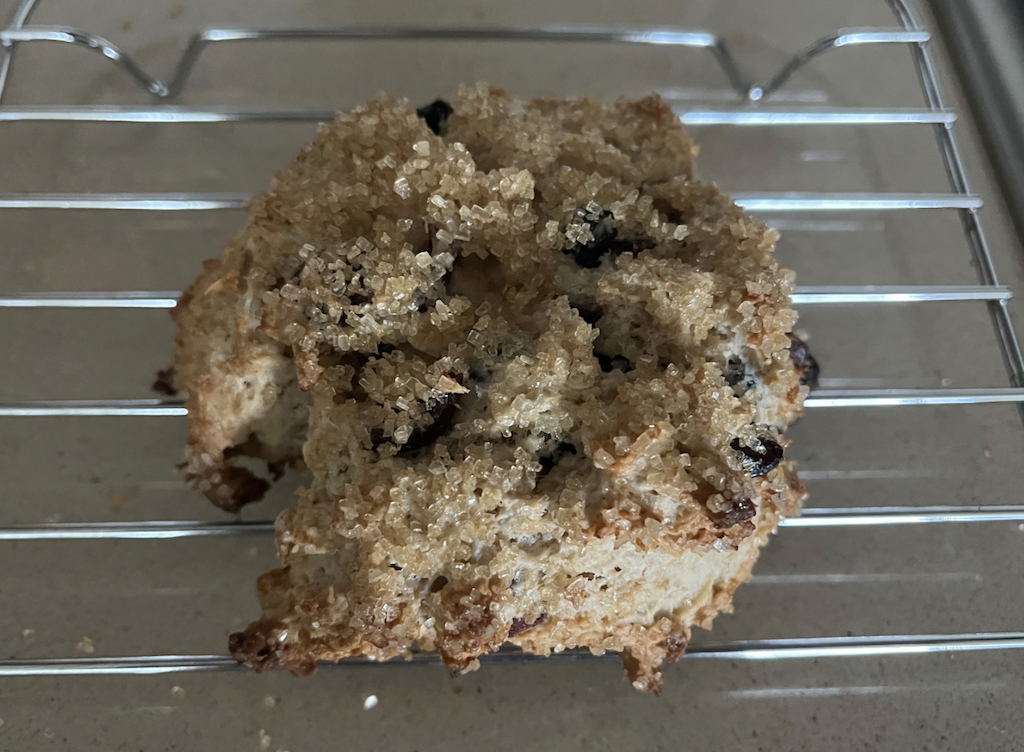
\includegraphics{./assets/scone.png}

\bookmarksetup{startatroot}

\hypertarget{dinner}{%
\chapter*{Dinner}\label{dinner}}
\addcontentsline{toc}{chapter}{Dinner}

\markboth{Dinner}{Dinner}

\hypertarget{brisket}{%
\section*{Brisket}\label{brisket}}
\addcontentsline{toc}{section}{Brisket}

\markright{Brisket}

\begin{itemize}
\tightlist
\item
  3 to 5 pound trimmed brisket
\item
  1 jar chili sauce (Bennet's preferred)
\item
  Low sodium chicken broth or water (1/2 cup or so)
\item
  1 or 2 yellow onions depending on size
\item
  Optional 1 tablespoon tamarind paste ¨ Time
\end{itemize}

Slice onions and put in a layer in the bottom of a deep pan. Put chili
sauce in a bowel. Rinse jar with broth or water and add. Stir in
tamarind paste if desired. Pour over brisket and cover with top or
tented tinfoil. Place pan on baking tray and cook at 325 degrees for 5
to 6 hours or until fork moves freely in brisket. Let cool and then
remove from pan and liquid onion mixture to refrigerate. Put onions and
liquid in a container and refrigerate overnight. Remove fat from top and
blend as desired into gravy. Slice the cooled brisket, put into oven
safe container, and cover with gravy. Freeze for at least 24 hours.
Reheat at 325 degrees for 1 to 2 hours.

\hypertarget{next}{%
\section*{Next}\label{next}}
\addcontentsline{toc}{section}{Next}

\markright{Next}

\bookmarksetup{startatroot}

\hypertarget{desert}{%
\chapter*{Desert}\label{desert}}
\addcontentsline{toc}{chapter}{Desert}

\markboth{Desert}{Desert}

\hypertarget{blueberry-almond-and-lemon-cake-yotam-ottolenghi}{%
\section*{Blueberry Almond and Lemon Cake (Yotam
Ottolenghi)}\label{blueberry-almond-and-lemon-cake-yotam-ottolenghi}}
\addcontentsline{toc}{section}{Blueberry Almond and Lemon Cake (Yotam
Ottolenghi)}

\markright{Blueberry Almond and Lemon Cake (Yotam Ottolenghi)}

\begin{itemize}
\tightlist
\item
  1/2 cup (1 stick) plus 3 tablespoons unsalted butter, room temperature
\item
  3/4 to 1 cup granulated sugar
\item
  1 teaspoon lemon zest
\item
  1 tablespoon lemon juice
\item
  1 teaspoon vanilla extract
\item
  3 large eggs, beaten
\item
  2/3 cup allpurpose flour sifted
\item
  1 1/4 teaspoons baking powder -
\item
  1/8 teaspoon salt
\item
  1 cup almond flour
\item
  1 1/2 cups fresh blueberries
\item
  2/3 cup confectioners' sugar
\end{itemize}

Heat oven to 375 and grease a 9 or 8 inch loaf pan with butter; line
with a parchment paper sling and butter the paper. Beat butter, sugar,
lemon zest and vanilla extract in bowl at high speed for 3 to 4 minutes;
lower to medium; add eggs one at a time. In a separate bowl, whisk
flour, baking powder, salt and almond flour. Add to mixer in parts until
just mixed. Fold in about 3/4 of the blueberries by hand, then scoop
batter into the prepared loaf pan. Bake 15 minutes; sprinkle the
remaining blueberries over the top of the cake. Bake for 5 to 20 minutes
more until golden brown but still uncooked. Cover loosely with foil and
bake 25 to 30 minutes more. Remove from oven and set aside in its pan to
cool for 10 minutes then place on a wire rack to cool. Add lemon juice
and icing sugar to a bowl and whisk together until smooth; pour over the
cake and gently spread.

\hypertarget{chocolate-chip-cookies}{%
\section*{Chocolate Chip Cookies}\label{chocolate-chip-cookies}}
\addcontentsline{toc}{section}{Chocolate Chip Cookies}

\markright{Chocolate Chip Cookies}

(based on
\href{https://cooking.nytimes.com/recipes/1015819-chocolate-chip-cookies}{Jacques
Torres})

\begin{itemize}
\tightlist
\item
  8 1/2 ounces cake flour
\item
  6 1/2 ounces bread flour
\item
  2 ounces almond flour (or use 8 1/2 bread flour)
\item
  1/2 teaspoon baking powder
\item
  1/2 teaspoon baking soda
\item
  1 teaspoon salt (as desired)
\item
  1 1/4 cups unsalted butter
\item
  9 ounces brown sugar
\item
  7 ounces granulated sugar
\item
  1/4 cup granulated sugar
\item
  2 large eggs
\item
  2 teaspoons vanilla extract
\item
  1 to 1 1/4 pounds bittersweet chocolate disks
\end{itemize}

Sift flours, baking soda, baking powder, and salt. Cream butter and
sugars at high speed until very light (about 5 minutes). Add eggs one at
a time. At low speed mix in dry ingredients until just combined. Turn
mixer off and remove paddle. Mix in chocolate disks slowly by hand.
Scoop into 3 1/2 ounce balls and refrigerate for 24 hours. Bake in a
convection oven at 350 for 10 to 12 minutes.

\begin{figure}

{\centering \includegraphics{./assets/torres.png}

}

\caption{Made with Belcolade chocolate disks.}

\end{figure}

\bookmarksetup{startatroot}

\hypertarget{bread}{%
\chapter*{Bread}\label{bread}}
\addcontentsline{toc}{chapter}{Bread}

\markboth{Bread}{Bread}

\hypertarget{isabelles-challah}{%
\section*{Isabelle's Challah}\label{isabelles-challah}}
\addcontentsline{toc}{section}{Isabelle's Challah}

\markright{Isabelle's Challah}

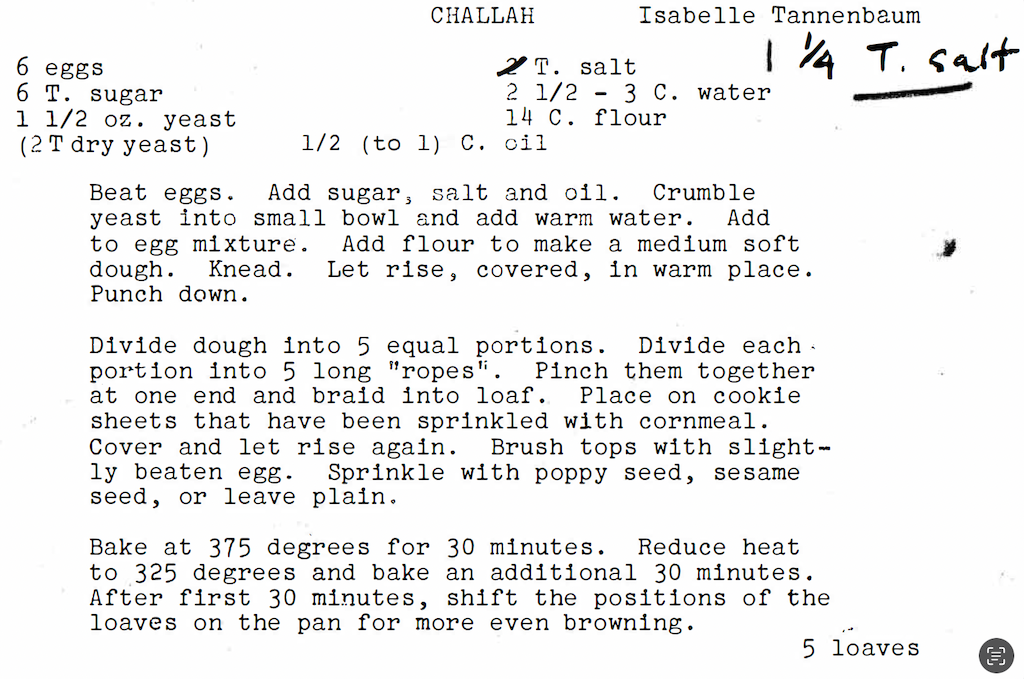
\includegraphics{./assets/challah_recipe.png}

\includegraphics{./assets/challahPhotoRound.png}

\hypertarget{next-1}{%
\section*{Next}\label{next-1}}
\addcontentsline{toc}{section}{Next}

\markright{Next}



\end{document}
